%\documentclass{article}
\documentclass{article}
\usepackage{tikz}
\usepackage{tikz-dependency}
\usepackage{multirow}
\usepackage{caption} 
\captionsetup[table]{skip=10pt}
\usepackage{array}
\newcolumntype{C}[1]{>{\centering\let\newline\\\arraybackslash\hspace{0pt}}m{#1}}
\usepackage[T1]{fontenc}




\begin{document}

\begin{table}
  [ht] 
   \begin{tabular}{ c  | c | l   r } \hline 
%      catena &  type & \hspace{1cm}HI \hspace{2.8cm}Mixed & HF \hspace{1cm} \\
catena &  type & \multicolumn{2}{l}{\hspace{1cm} HI\hspace{3cm} Mixed\hspace{3cm} HF} \\
       \hline \multirow{2}{*}{parallel} & adverbs & \parbox[c]{14em}{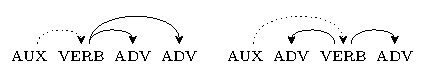
\includegraphics[width=5cm, height=1.5cm]{adverbs/ADV_ADV_V_HI.pdf}} & \parbox[c]{14em}{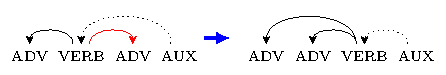
\includegraphics[width=5cm, height=1.5cm]{adverbs/ADV_ADV_V_HF.pdf}} \\
    & adjectives & \parbox[c]{14em}{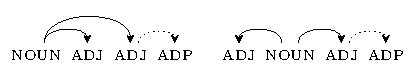
\includegraphics[width=5cm, height=1.5cm]{adjectives/ADJ_ADJ_N_HI.pdf}} & \parbox[c]{14em}{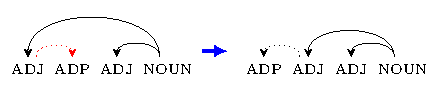
\includegraphics[width=5cm, height=1.5cm]{adjectives/ADJ_ADJ_N_HF.pdf}} \\
    \hline
  \end{tabular}
\end{table}

\end{document}